\documentclass{article}
\usepackage{mystyle}
\title{Open Economic Model}

\begin{document}
    \maketitle

    Homework 2 problem 19 looks something like this for y'all.
    \\
    \begin{centering}
        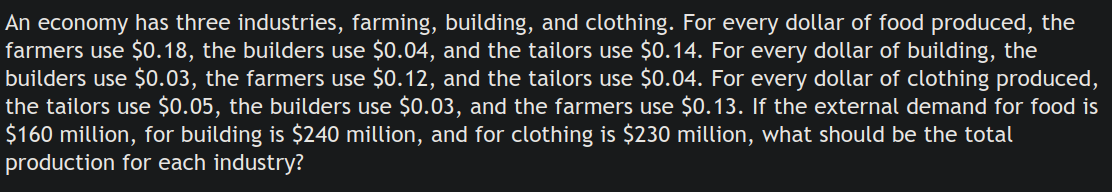
\includegraphics[width=\textwidth]{images/HW2Prob19.png}
    \end{centering}

    This problem is a little different than the type we covered in class. We assumed that we would
    be using all of our output internally. However, this problem requires us to have a certain 
    amount of net production to sell (Think of this like budgeting in savings in your monthly expenses.
    While your food or gas bill will depend on how much you exercise and how much drive, a savings
    goal is static).

    More information on this problem can be found with the 
    \href{https://lyryx.com/wp-content/uploads/2018/01/Nicholson-OpenLAWA-2018A.pdf}{Linear Algebra
    With Applications} textbook on page 137. Note: This is later in the book than we currently are
    so some of the vocabulary and things they prove are things we won't worry about yet!

    For the example above, we first set up our system as follows where $p_f$ denotes the amount
    of money produced from farming, $p_b$ denotes the amount of money produced from building, and
    $p_c$ denotes the amount of money produced from clothing. Since we are given part of our data in
    millions, we will use millions of dollars as our units.


    \begin{align*}
        p_f &= \textnormal{Cost of production} + \textnormal{External demand} = (.18p_f + .12p_b + .13p_c) + 160\\
        p_b &= \textnormal{Cost of production} + \textnormal{External demand} = (.04p_f + .03p_b + .03p_c) + 240\\
        p_c &= \textnormal{Cost of production} + \textnormal{External demand} = (.14p_f + .04p_b + .05p_c) + 230
    \end{align*}
    Which can be rearranged as below
    \begin{align*}
        .82p_f - .12p_b - .13p_c &= 160\\
       -.04p_f + .97p_b - .03p_c &= 240\\
       -.14p_f - .04p_b + .95p_c &= 230
    \end{align*}
    Giving us the following augmented matrix
    \[
        \aMat{ccc|c}{
                .82 & -.12 & -.13 & 160 \\
                -.04& .97  & -.03 & 240 \\
                -.14& -.04 & .95  & 230
        }
    \]
    This is a bit of a pain to perform our row reductions due to the decimals and the size of
    the numbers. I won't ask you to do one like this by hand on the written homework or on an exam.
    If this happens again in a future homework, you can use python to reduce the matrix if it doesn't
    play nice with a couple steps for the MyOpenMath assignments (I'll also make this announcement
    in class).
    
    The python to reduce this matrix and give us RREF is below
    \begin{verbatim}
import sympy as sym
A = sym.Matrix([[.82, -.12, -.13, 160],[-.04, .97, -.03, 240],[-.14, -.04, .95, 230]])
display(A) # To double check we input the matrix correctly
[RREF, pivots] = A.rref() # Stores the RREF form in RREF and the pivot information in pivots
display(RREF[:,3]) # Prints out the right hand side
    \end{verbatim}
    Which gives us the output
    \[
        \begin{bmatrix}
            281.100694254633\\268.132619034603\\294.820423112666
        \end{bmatrix}
    \]
    Note: Computers can't do math exactly like we can, so this might be a little different than
    if you were to do it by hand, so we'd round to 2 decimal points, and it'll be good enough for
    our uses.
    \[
        \begin{bmatrix}
            281.10\\268.13\\294.82
        \end{bmatrix}
    \]
\end{document}
